% XCircuit output "lms7_vna.tex" for LaTeX input from lms7_vna.ps
\def\putbox#1#2#3#4{\makebox[0in][l]{\makebox[#1][l]{}\raisebox{\baselineskip}[0in][0in]{\raisebox{#2}[0in][0in]{\scalebox{#3}{#4}}}}}
\def\rightbox#1{\makebox[0in][r]{#1}}
\def\centbox#1{\makebox[0in]{#1}}
\def\topbox#1{\raisebox{-0.60\baselineskip}[0in][0in]{#1}}
\def\midbox#1{\raisebox{-0.20\baselineskip}[0in][0in]{#1}}
   \scalebox{1}{
   \normalsize
   \parbox{10.1771in}{
   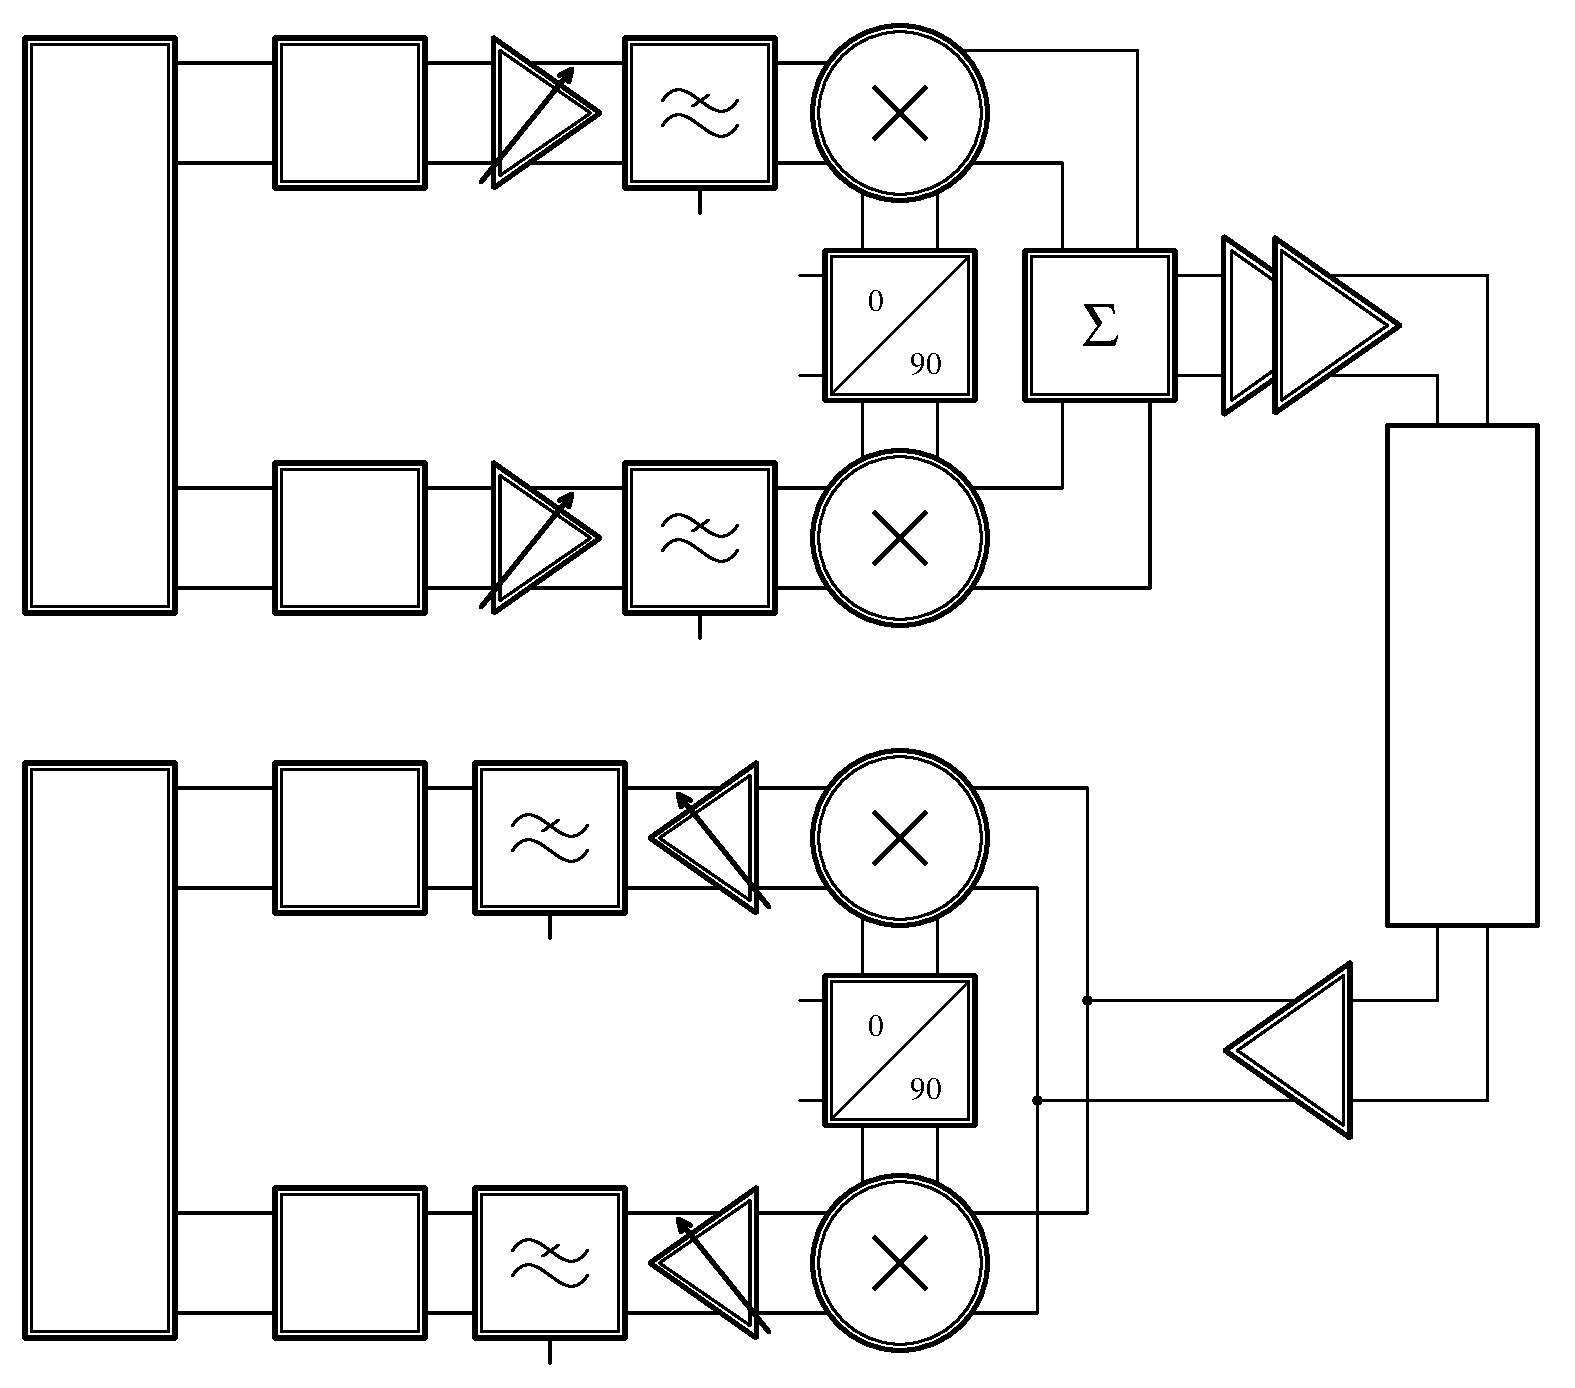
\includegraphics[scale=1]{lms7_vna}\\
   % translate x=1584 y=1104 scale 0.38
   \putbox{8.56in}{7.81in}{2.40}{\centbox{\midbox{TX PAD}}}%
   \putbox{8.56in}{2.97in}{2.40}{\centbox{\midbox{LNA}}}%
   \putbox{2.22in}{8.39in}{2.40}{\centbox{\midbox{DAC}}}%
   \putbox{2.22in}{5.56in}{2.40}{\centbox{\midbox{DAC}}}%
   \putbox{2.22in}{3.56in}{2.40}{\centbox{\midbox{ADC}}}%
   \putbox{2.22in}{0.72in}{2.40}{\centbox{\midbox{ADC}}}%
   \putbox{0.56in}{6.97in}{3.60}{\rotatebox{-270}{\centbox{\midbox{TxTSP}}}}%
   \putbox{0.56in}{2.14in}{3.60}{\rotatebox{-270}{\centbox{\midbox{RxTSP}}}}%
   \putbox{1.35in}{8.39in}{1.80}{\centbox{\midbox{TXI}}}%
   \putbox{1.39in}{5.56in}{1.80}{\centbox{\midbox{TXQ}}}%
   \putbox{1.35in}{3.56in}{1.80}{\centbox{\midbox{RXI}}}%
   \putbox{1.39in}{0.72in}{1.80}{\centbox{\midbox{RXQ}}}%
   \putbox{5.22in}{6.97in}{2.40}{\rightbox{\midbox{LO from TX PLL}}}%
   \putbox{5.22in}{2.14in}{2.40}{\rightbox{\midbox{LO from TX PLL}}}%
   \putbox{9.64in}{4.47in}{2.40}{\centbox{$\phi$}}%
   } % close 'parbox'
   } % close 'scalebox'
   \vspace{-\baselineskip} % this is not necessary, but looks better
